%%%%%%%%%%%%%%%%%%%%%%%%%%%%%%%%%%%%%%%%%
% University Assignment Title Page 
% LaTeX Template
% Version 1.0 (27/12/12)
%
% This template has been downloaded from:
% http://www.LaTeXTemplates.com
%
% Original author:
% WikiBooks (http://en.wikibooks.org/wiki/LaTeX/Title_Creation)
%
% License:
% CC BY-NC-SA 3.0 (http://creativecommons.org/licenses/by-nc-sa/3.0/)
% 
% Instructions for using this template:
% This title page is capable of being compiled as is. This is not useful for 
% including it in another document. To do this, you have two options: 
%
% 1) Copy/paste everything between \begin{document} and \end{document} 
% starting at \begin{titlepage} and paste this into another LaTeX file where you 
% want your title page.
% OR
% 2) Remove everything outside the \begin{titlepage} and \end{titlepage} and 
% move this file to the same directory as the LaTeX file you wish to add it to. 
% Then add \input{./title_page_1.tex} to your LaTeX file where you want your
% title page.
%
%%%%%%%%%%%%%%%%%%%%%%%%%%%%%%%%%%%%%%%%%
%\title{Title page with logo}
%----------------------------------------------------------------------------------------
%   PACKAGES AND OTHER DOCUMENT CONFIGURATIONS
%----------------------------------------------------------------------------------------

\documentclass[12pt]{report}
\usepackage[english]{babel}
\usepackage[utf8x]{inputenc}
\usepackage{amsmath}
\usepackage{graphicx}
\usepackage[colorinlistoftodos]{todonotes}
\usepackage{float}
\usepackage{hyperref}
\begin{document}

\begin{titlepage}

\newcommand{\HRule}{\rule{\linewidth}{0.2mm}} % Defines a new command for the horizontal lines, change thickness here

\center % Center everything on the page
 
%----------------------------------------------------------------------------------------
%   HEADING SECTIONS
%----------------------------------------------------------------------------------------

%\textsc{\LARGE EURECOM}\\[1.5cm] % Name of your university/college
\textsc{\Large Semester Project Report}\\[0.5cm] % Major heading such as course name
\textsc{\large Department Of Data Science and Engineering}\\[0.5cm] % Minor heading such as course title

%----------------------------------------------------------------------------------------
%   TITLE SECTION
%----------------------------------------------------------------------------------------

\HRule \\[0.4cm]
{ \Large \bfseries Emotion Patterns in Music Playlists}\\[0.4cm] % Title of your document
\HRule \\[6cm]
 
%----------------------------------------------------------------------------------------
%   AUTHOR SECTION
%----------------------------------------------------------------------------------------

\begin{minipage}{0.4\textwidth}
\begin{flushleft} \large
\emph{Authors:}\\
Sara \textsc{Giammusso} \\ Mario \textsc{Guerriero} % Your name
\end{flushleft}
\end{minipage}
~
\begin{minipage}{0.4\textwidth}
\begin{flushright} \large
\emph{Supervisors:} \\
Raphael \textsc{Troncy}\\ Pasquale \textsc{Lisena}\\ Enrico \textsc{Palumbo} % Supervisor's Name
\end{flushright}
\end{minipage}\\[2cm]

% If you don't want a supervisor, uncomment the two lines below and remove the section above
%\Large \emph{Author:}\\
%John \textsc{Smith}\\[3cm] % Your name

%----------------------------------------------------------------------------------------
%   DATE SECTION
%----------------------------------------------------------------------------------------

{\large \today}\\[2cm] % Date, change the \today to a set date if you want to be precise

%----------------------------------------------------------------------------------------
%   LOGO SECTION
%----------------------------------------------------------------------------------------


\includegraphics[width=0.3\textwidth]{logo.png}\\[1cm] % Include a department/university logo - this will require the graphicx package
 
%----------------------------------------------------------------------------------------

\vfill % Fill the rest of the page with whitespace

\end{titlepage}

\tableofcontents


\begin{abstract}

Music streaming services such as Spotify are revolutionizing the music world, enabling a transition from artist-created bundles of songs (CDs) to user-created playlists.\par
Different logics may be applied in the generation of a playlist: they can contain songs of a similar genre (e.g. ``Rock playlist''), fit to a particular occasion (e.g. ``New year's eve party''), to a particular context (e.g. ``Gym''), to a particular mood (e.g.``Happy'') and so on.\par

The goal of this semester project is to unravel the emotion patterns underlying the sequences of songs in a playlist using automatic approaches of Emotion Detection on the lyrics.

\end{abstract}
\newpage

% CHAPTER 1 - INTRODUCTION
\chapter{Introduction}
\section{Background}
In the last few years the online music streaming services such as Spotify, Apple Music and Deezer introduced, among others,  the possibility to create playlists thus opening new challenges on music recommendation.\par
One of the new possible tasks a modern Recommender System should perform is automatic playlist continuation. By suggesting appropriate songs to add to a playlist, a Recommender System can increase user engagement by making playlist creation easier, as well as extending listening beyond the end of existing playlists. \par
More precisely the task of automatic playlist continuation consists in: given a set of playlist features, the system shall generate a list of recommended tracks that can be added to that playlist, thereby ``continuing'' the playlist. \par

In fact, one of the final goals of this project was to produce numerical features to be used in a recommender system for music playlists. Specifically, this recommender system had to be built for the RecSys Challenge 2018\footnote{\url{https://recsys-challenge.spotify.com/}}, hosted for this year by Spotify, which provided a huge dataset of a milion playlist coming from their own platform. Since the goal of this challenge is to improve the playlist continuation feature of the Spotify's recommender system, we believed that putting emotions in the features used to group playlists could be useful for achieving better performances. For this reason, the output of this system is a vector where, each element, expresses the likelihood score for the releated emotion. The details of how this vector is built will be made clearer throughout this report.

\section{Project scope}

One of the possible features to consider in developing a system for the automatic playlist continuation task is the emotion expressed in each song of the playlist and the more frequent transition patterns from one emotion to the other. Thus, not only the emotion of each song lyrics must be detected, but also the transitions between emotions must be analyzed. \par
Emotion Detection is a novel and promising field of study of Natural Language Understanding, which is able to automatically infer what are the emotions expressed in a text. It can be considered as a Sentiment Analysis task, which is the computational treatment of opinions, sentiments and subjectivity of a natural language text. \par

\section{Results}

Below we just reported the accuracy results we obtained throughout our project while classifying emotions both in song lyrics and in playlists, as shown in table \ref{tab:compar} and \ref{tab:compar2} respectively.

\begin{table}[H]
\centering
\begin{tabular}{ |p{3cm}||p{1.5cm}|p{1.5cm}|p{1.5cm}|p{1.5cm}|  }
 \hline
 \multicolumn{5}{|c|}{10-fold Cross Validation Accuracy} \\
 \hline
 Dataset & ANN & LR &SVM & xgboost\\
 \hline
MoodyLyrics  & 90.55\%    &- &  90\% & 86\%\\
MoodyLyrics4Q  & 58.45\%    &57.87\% &  58.04\% & 56.89\%\\
Both together &   68.41\%  & 69.42\%   &69.32\% &64.27\%\\
\hline
\end{tabular}
\caption{Emotion detection accuracies on lyrics} \label{tab:compar}
\end{table}

\begin{table}[H]
\centering
\begin{tabular}{ |p{3cm}||p{1.5cm}|p{1.5cm}| }
 \hline
 \multicolumn{3}{|c|}{Playlist Classification Accuracy} \\
 \hline
Dataset & With outliers & Without outliers\\
 \hline
MoodyLyrics & 29\% & 29\%\\
MoodyLyrics4Q  & 66\%    &66\%\\
Both together &   50\%  & 47\%\\
\hline
\end{tabular}
\caption{Playlist classification accuracies} \label{tab:compar2}
\end{table}

We will go into the details of how those results were obtained in the next chapters of this report.

\section{Emotion Classification Utilities}

The above results can be obtained using the code which can be found in the project's GitHub repository\footnote{\url{https://github.com/sgiammy/emotion-patterns-in-music-playlists}}. Specifically, using this code, we can perform classification at three different levels:
\begin{itemize}
\item \textbf{Lyrics level}: using the function \texttt{classify(sid, artist, title)} of the \texttt{src\/emoclassify.py} script
\item \textbf{Playlist level}: using the function \texttt{robust\_classify(playlist\_vect)} from the \texttt{src\/playlist\_classify.py} script
\item \textbf{Spotify's dataset slice level}: using the function \texttt{classify\_slice(slice\_path)} from the \texttt{src\/slice\_classify.py} script
\end{itemize}

Along with those utilitiy programs we also provided some pre-trained models in the folder \texttt{src\/model}, which can be used to reproduce the results we obtained. The details of how those models were built will be discussed later in this report.

\section{Report outline}

The report is structured as follow: \textit{chapter 2} contains the analysis of the state of the art in emotion detection tasks. \textit{Chapter 3} includes an exploration of the background knowledge for this project, \textit{chapter 4} describes the lyrics emotion classification approaches tried, \textit{chapter 5} the playlists classification methods and results while \textit{chapter 6} contains conclusions and future works considerations. 
\chapter{The State of the Art}

In the following chapter we will briefly go through the knowledge we acquired while exploring already existing materials in the same context of our problem.

\section{Sentiment Analysis} 
Sentiment Analysis (SA) is the computational study of people's opinions, attitudes and emotions toward an entity, the entity being an individual, event or topic.\cite{survey} \par

Sentiment Analysis can be considered a classification task as illustrated in Fig \ref{fig:sa_process}.\\

\begin{figure}[H]
\centering
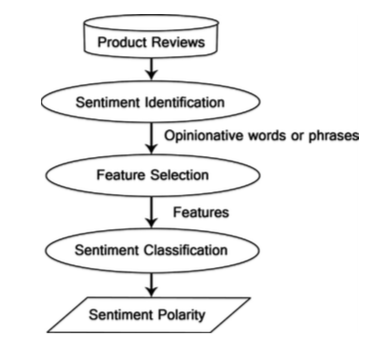
\includegraphics[width=0.4\textwidth]{./chapters/chapter1/images/sa_process}
\caption{Sentiment analysis process on product reviews\cite{survey}}
\label{fig:sa_process}
\end{figure}

There are three main classification levels in SA: 
\begin{itemize}
\item Document-level
\item Sentence-level
\item Aspect-level
\end{itemize}
Their difference is the granularity at which they operate. Indeed, while document-level SA aims to classify a document as expressing a positive or negative opinion or sentiment by considering the whole document as the basic information unit, sentence-level SA aims at classifying the sentiments/opinions expressed in each sentence.
In both cases the first step is to identify whether the sentence/document is subjective or objective and if it is subjective determine whether the sentence expresses positive or negative opinions. \par

In certain applications, classifying text at the document level or at the sentence level may not provide the necessary details needed for detecting opinions on all aspects of the entity. Aspect-level SA, instead, aims at classifying the sentiment with respect to the specific aspects of entities. The first step is to identify the entities and their aspects. Then, all the different opinions on the same entity must be considered. Indeed, the opinion holders may also give different opinions for different aspects of the same entity, e.g. ``This chair is ugly but it is comfortable''.

Sentiment Analysis task is considered as a sentiment classification (SC) problem. The first step in the SC problem is to extract and select text features. Some of the most commonly used features are:
\begin{itemize}
\item \textbf{Terms presence and frequency}: These features are individual words or word n-grams and their frequency counts;
\item \textbf{Parts of speech (POS)}: finding adjectives, pronouns, etc. as they are important indicators of opinions;
\item \textbf{Opinion words and phrases}: these are words commonly used to express opinions including \textit{good or bad, like or hate}. On the other hand, some phrases express opinions without using opinion words, e.g. \textit{cost me and arm and a leg};
\item \textbf{Negations}: the appearance of negative words may change the opinion orientation like \textit{not good} is equivalent to \textit{bad}. 
\end{itemize}

Sentiment Classification techniques can be roughly divided into machine learning approach, lexicon based approach and hybrid approach\cite{survey}. \par

The \textit{Machine Learning Approach (ML)} applies the famous ML algorithms and uses linguistic features. 

The \textit{Lexicon-based Approach} relies on a sentiment lexicon, a collection of known and precomiled sentiment terms. It is divided into dictionary-based approach and corpus-based approach which use statistical or semantic methods to find sentiment polarity.

The \textit{Hybrid Approach} combines both approaches. 

The various approaches and the most popular algorithms of SC are illustrated in Fig \ref{fig:sentiment_classification}. 

\begin{figure}[H]
\centering
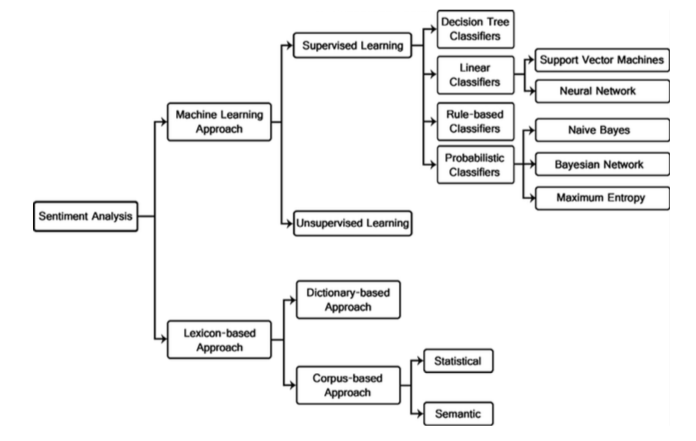
\includegraphics[width=0.8\textwidth]{./chapters/chapter1/images/sentiment_classification}
\caption{Sentiment classification techniques\cite{survey}}
\label{fig:sentiment_classification}
\end{figure}

The text classification methods using ML approach can be roughly divided into supervised and unsupervised learning methods. The supervised methods make use of a large number of labeled training documents. The unsupervised methods are used when it is difficult to find these labeled training training documents. \par
The lexicon-based approach depends on finding the opinion lexicon which is used to analyze the text. There are two methods in this approach:

\begin{itemize}
\item Dictionary-based
\item Corpus-based
\end{itemize}

In the Dictionary-based approach a small set of opinion words is collected manually with known orientations. Then, this set is grown by searching their synonyms and antonyms. The newly found words are added to the seed list then the next iteration starts. The iterative process stops when no new words are found. The dictionary based approach has a major disadvantage which is the inability to find opinion words with domain and context specific orientation. 

The limitation of the dictionary-based approach is addressed by the corpus-based approach, which depends on syntactic patterns or patterns that occur together along with a seed list of opinion words to find other opinion words in a large corpus. One of these methods is called \textit{sentiment consistency}: it starts with a list of seed opinion adjectives, and used them along with a set of linguistic constraints to identify additional adjective opinion words and their orientations. The constraints being for example \textit{AND, OR, BUT, EITHER-OR,...}; the conjunction \textit{AND} for example says that conjoined adjectives usually have the same orientation. \par

\section{Emotion Detection}

Emotion detection (ED) is the process of identifying human emotions. It is a recent field of research that is closely related to Sentiment Analysis. Indeed, Sentiment Analysis aims to detect positive, neutral or negative feelings from text, whereas Emotion Analysis aims to detect and recognize feelings in natural language texts. Therefore we can look at ED as a finer grained task with respect to SA.\par
Emotion is expressed as joy, sadness, anger, surprise, hate, fear and so on. Since there is not any standard emotion word hierarchy, the focus is on the related research about emotion in cognitive psychology domain. In 2001, W. Gerrod Parrot, wrote a book named ``Emotions In Social Psychology''\cite{Parrott2016}, in which he explained the emotion system and formally classified the human emotions through an emotion hierarchy in six classes at primary level which are \textit{Love, Joy, Anger, Sadness, Fear and Surprise} \cite{edfromtext}.\par

Emotion detection may have useful applications, such as \cite{microsoft}: 
\begin{itemize}
\item Measure citizens happiness;
\item Pervasive computing: this may include suggesting help when anxiety is detected through speech, or to check the tone of an email; 
\item Improving perception of a customer to increase brand reputation and sales. 
\end{itemize}

Some of the biggest challenges in determining emotion are:
\begin{itemize}
\item \textit{Context-dependence of emotions}: people use different regulation strategies in different social contexts. A phrase can have element of \textit{anger} without using the word ``anger'' or any of its synonyms, e.g. \textit{``Shut up!''}
\item \textit{Word-sense disambiguation}: identifying which sense a word (i.e. its meaning) is used in a sentence, when the word has multiple meanings; 
\item \textit{Co-reference resolution}: pronouns and other referring expressions must be connected to the right individuals;
\item Lack of labelled emotion databases. 
\end{itemize}

The main methods used for text based emotion detection are: 
\begin{itemize}
\item \textit{Keyword Spotting}
\item \textit{Lexical Affinity}
\item \textit{Learning-based}
\item \textit{Hybrid}
\end{itemize}

\paragraph{Keyword Spotting}
The keyword pattern matching problem can be described as the problem of finding occurrences of keywords from a given set as substrings in a given string. These words are classified into categories such as disgusted, sad, happy, angry, fearful, surprised, etc. The process of Keyword spotting method is  shown in Fig \ref{fig:keyword_spotting}. 

\begin{figure}[H]
\centering
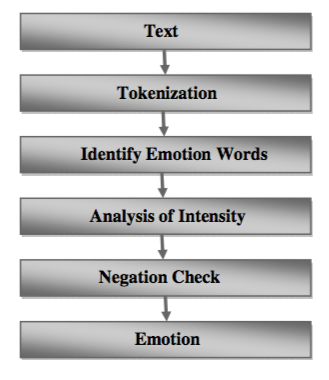
\includegraphics[width=0.4\textwidth]{./chapters/chapter1/images/keyword_spotting}
\caption{Keyword spotting technique}
\label{fig:keyword_spotting}
\end{figure}

The first step is converting data into tokens, i.e. a sentence into words, then from these tokens emotion words are detected. The second step is analyzing the intensity of emotion words. Sentence, then, is checked whether negation is involved in it or not then finally an emotion class will be assigned.

\paragraph{Lexical Affinity method} 
The Lexical Affinity approach is an extension of keyword spotting technique: apart from picking up emotional keywords it assigns \textit{probabilistic affinity} for a particular emotion to arbitrary words. This technique has the main disadvantage of missing out emotion content that resides deeper than the word level.\\
For example the word 'accident', having been assigned a high probability of indicating a negative emotion, would not contribute correctly to the emotional assessment of phrases like \textit{``I avoided an accident''} or \textit{``I met my girlfriend by accident''}. 

\paragraph{Learning-based methods}
Learning-based methods change the focus from ``determining emotions'' to ``classify the input texts into different emotions''. Indeed, learning-based methods try to detect emotions based on a previously trained classifier, which apply various theories of machine learning such as Support Vector Machines (SVMs).

\paragraph{Hybrid Methods}
Since keyword-based methods and na\"{i}ve learning-based methods could not acquire satisfactory results, some systems use hybrid approach by combining both keyword spotting technique and learning based method, which help to improve accuracy. \\
\\

However all these methods have some major limitations:
\begin{itemize}
\item \textit{Ambiguity in Keyword Definitions}: words can have multiple and vague meanings that can change according to different usages and contexts. Moreover emotion labels could have different emotions in some extreme cases such as ironic or cynical sentences; 
\item \textit{Lack of Linguistic Information}: these methods totally ignore syntax structures and semantics that also have influences on expressed emotions. For example the sentences \textit{``He laughed at me''} or \textit{``I laughed at him''} express two totally different meanings;
\item \textit{Incapability of Recognizing Sentences without Keywords}: sentences without any keyword would imply that they do not contain any emotion at all, which is obviously wrong. 
\end{itemize}

Deciding a way to label emotions is another challenging aspect of ED. There are mainly two possible ways to label data \cite{microsoft}:
\begin{enumerate}
\item The label is one between the set of emotions, e.g. \textit{anger, disgust, sad, happy, surpise, fear, neutral};
\item \textit{Slider approach}: the label is composed of percentages for each emotion, as described in Fig \ref{fig:emotion_labeling_sliders}.
\end{enumerate}

\begin{figure}[H]
\centering
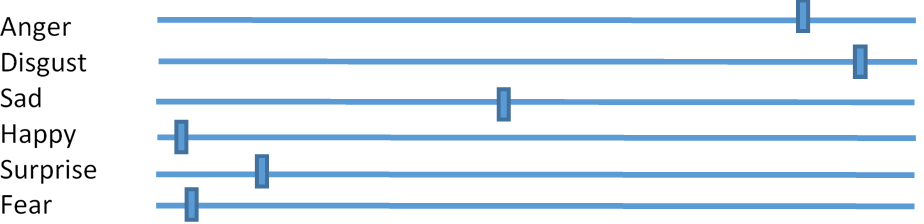
\includegraphics[width=0.8\textwidth]{./chapters/chapter1/images/emotion_labeling_sliders}
\caption{Slider approach\cite{microsoft}}
\label{fig:emotion_labeling_sliders}
\end{figure}

The sliders approach certainly offers more information but it comes with additional computational complications. However, the probabilistic assignment produced in the sliders approach can be turned into distinct labels of single emotions, just like those produced by first labeling approach, but of course, we can not move from the first approach to the second one. 


\chapter{Problem Pre-processing}
\section{The problem}
The goal of the semester project is to unravel the emotion pattern underlying the sequences of songs in a playlist using automatic approaches of Emotion Detection on the lyrics.\par
The problem can be divided into two main parts:
\begin{enumerate}
\item Classify emotions for each song based on the lyrics
\item Analyze emotion patterns in the playlists
\end{enumerate}

\section{Related work}
Emotion detection domain has already attracted many researchers from computer science, psychology, cognitive science and so on. \par
Before building our own emotion detection system we start analyzing some already existent classifier. \par
\paragraph{IBM Watson Natural Language Understanding}\cite{ibm_watson}
Watson is a question answering computer system capable of answering questions posed in natural language, developed by IBM.\par
Natural Language Understanding is a collection of APIs that allows to:
\begin{itemize}
\item Recognize the overall sentiment, in a scale from negative to positive [-1, 1];
\item Detect the emotion percentage between: joy, anger, disgust, sadness, fear;
\item Determine keywords ranked by relevance;
\item Extract entities: people, companies, organizations, cities and other information;
\item Classify content into hierarchical categories;
\item Identify general concepts that may not be directly referenced in the text; 
\end{itemize}
Results obtained analyzing Oasis - Wonderwall are illustrated in Fig.


\paragraph{IBM Watson Tone Analyzer}\cite{ibm_watson_tone}
It uses linguistic analysis to detect joy, fear, sadness, anger, analytical, confident, and tentative tones found in text. It allows to select different sources: tweets, online reviews, email messages, or other text. It uses both:
\begin{itemize}
\item the document level: to get a sense of the overall tone;
\item the sentence level: to identify specific areas where tones are the strongest.
\end{itemize}

\paragraph{QEmotion}\cite{qemotion}
Qemotion detects the main emotion of the speech and define the corresponding emotion in terms of temperature. 
\begin{itemize}
\item From $31^{\circ}$ to $40^{\circ}$ $\to$ Happiness
\item From $21^{\circ}$ to $30^{\circ}$ $\to$ Surprise
\item From $11^{\circ}$ to $20^{\circ}$ $\to $ Calm
\item From $6^{\circ}$ to $10^{\circ}$ $\to $ Fear
\item From $-5^{\circ}$ to $5^{\circ}$ $\to $ Sadness
\item From $-14^{\circ}$ to $-6^{\circ}$ $\to $ Anger
\item From $-20^{\circ}$ to $-15^{\circ}$ $\to $ Disgust
\end{itemize}


\section{NLP libraries}
In order to select the best Natural Language Processing library for our purpose we also analyzed pros and cons of the main Natural Language Processing libraries, i.e. NLTK, TextBlob, Standord's CoreNLP and SpaCy. 

\paragraph{NLTK: Natural Language Toolkit}
It is recommended only as an education and research tool. \\
Pros:
\begin{itemize}
\item its modularized structure makes it excellent for learning and exploring NLP concepts; 
\item over 50 corpora and lexicons, 9 stemmers, and a dozens of algorithms to choose from (this can also be considered as a con).
\end{itemize}
Cons: 
\begin{itemize}
\item Heavy library with a steep learning curve;
\item Slow and not production-ready. 
\end{itemize}

\paragraph{TextBlob}
Built on top on NLTK.\\
Pros: 
\begin{itemize}
\item More intuitive; 
\item Gentle learning curve. 
\end{itemize} 

\paragraph{Stanford's CoreNLP}
Java library with Python wrappers. \\
Pros:
\begin{itemize}
\item fast;
\item support for several major languages. 
\end{itemize}

\paragraph{SpaCy}
It is a new NLP library designed to be fast, streamlined and production-ready.\\
Pros:
\begin{itemize}
\item minimal number of options;
\item its philosophy is to only present the best algorithm for each purpose. 
\end{itemize}
Cons:
\begin{itemize}
\item it is new, so its support community is not as large as other libraries, but it is growing very fast.
\end{itemize}





\section{Word embedding techniques}
Word embeddings are a set of feature learning techniques mapping words or phrases from the vocabulary to vectors or real numbers. \par
These techniques map sparse word vectors into continuous space based on the surrounding context. For example if \textit{``salt''} and \textit{``seasoning''} appear within the same context, the model will indicate that \textit{``salt''} is conceptually closer to \textit{``seasoning''}, than another word, say \textit{``chair''}.\par
There are two main embedding libraries: Word2vec and FastText. While Word2vec treats each word in corpus like an atomic entity generating a vector for each word, FastText treats each word as composed of character ngrams, so the vector for a word is made of the sum of this character n grams. \par
For example,  the word vector \textit{``apple''} is a sum of the vectors of the n-grams ``ap'', ``app'', ``appl'', ``apple'', ``ppl', ``pple'', ``ple'', ``le'' assuming 3 and 6 as minimum and maximum ngrams size.\\
The difference between Word2vec and FastText manifests as follows:
\begin{enumerate}
\item \textit{Rare words}: even if words are rare, their character n-grams are still shared with other words - hence the embeddings with FastText can still be good;
\item \textit{Out of vocabulary words}: FastText can construct the vector for a word from its character n-grams even if word does not appear in training corpus;
\item \textit{Hyperparameters choice}: FastText requires to  choose the minimum and maximum n-grams sizes, and this directly impacts the computation time and the memory requirements. 
\end{enumerate}




\section{Public datasets}
A big challenge in emotion detection is the lack of a labelled emotion database to enable active innovation. Currently, few publicly accessible databases are available.\\\textit{MoodyLyrics}\cite{moodylyrics} contains around 2500 songs manually annotated through Amazon Mechanical Turk with 4 different emotion, i.e., happy, sad, angry and relaxed.\\
\textit{EmoInt}\cite{emoint} contains manually annotated tweets classified according to the intensities of anger, fear, joy and sadness. \textit{EmoBank}\cite{emobank} instead contains 10.000 sentences, each of which has been annotated according to both the emotion expressed by the writer and the emotion perceived by the reader. 

















\begin{thebibliography}{9}
\bibitem{survey} 
Walaa Medhat, Ahmed Hassan, and Hoda Korashy. \textit{Sentiment Analysis Algorithms and Applications: A Survey}. Ain Shams Engineering Journal, 1994.
 
\bibitem{edfromtext} 
Shiv Naresh Shivhare1 and Prof. Saritha Khethawat. \textit{Emotion Detection From Text}, 2012.

 
\bibitem{microsoft} 
Emotion detection and recognition from text using Deep Learning,
\\\href{https://www.microsoft.com/developerblog/2015/11/29/emotion-detection-and-recognition-from-text-using-deep-learning/}{link}

 
\bibitem{ibm_watson} 
IBM Watson: Natural Language Understanding APIs
\\\footnotesize \url{https://www.ibm.com/watson/services/natural-language-understanding/}

\bibitem{ibm_watson_tone} 
IBM Watson: Tone Analyzer
\\\footnotesize \url{https://www.ibm.com/watson/services/tone-analyzer/}

\bibitem{qemotion} 
QEmotion
\\\footnotesize \url{http://www.qemotion.com/demo.php}

\bibitem{moodylyrics} 
MoodyLyrics: A Sentiment Annotated Lyrics Dataset
\\\footnotesize \url{https://www.researchgate.net/publication/317031495_MoodyLyrics_A_Sentiment_Annotated_Lyrics_Dataset}

\bibitem{emoint} 
Shared Task on Emotion Intensity (EmoInt)
\\\footnotesize \url{http://saifmohammad.com/WebPages/EmotionIntensity-SharedTask.html}

\bibitem{emobank} 
EmoBank
\\\footnotesize \url{https://github.com/JULIELab/EmoBank}

\bibitem{features}
Fell, Michael and Caroline Sporleder. "Lyrics-based Analysis and Classification of Music." COLING (2014).

\bibitem{spacy}
SpaCy - Industrial-Strength Natural Language Processing in Python
\\\footnotesize \url{https://spacy.io/}

\bibitem{word2vec}
word2vec - Tool for computing continuous distributed representations of words
\\\footnotesize \url{https://code.google.com/archive/p/word2vec/}

\bibitem{textblob}
TextBlob: Simplified Text Processing
\\\footnotesize \url{http://textblob.readthedocs.io/en/dev/index.html}

\end{thebibliography}
 

\end{document}
              